\documentclass[amsmath, amssymb, aip, jmp, reprint]{revtex4-2}
\usepackage{tikz}
\usetikzlibrary{shapes.geometric}
\usetikzlibrary{decorations.markings}

\begin{document}

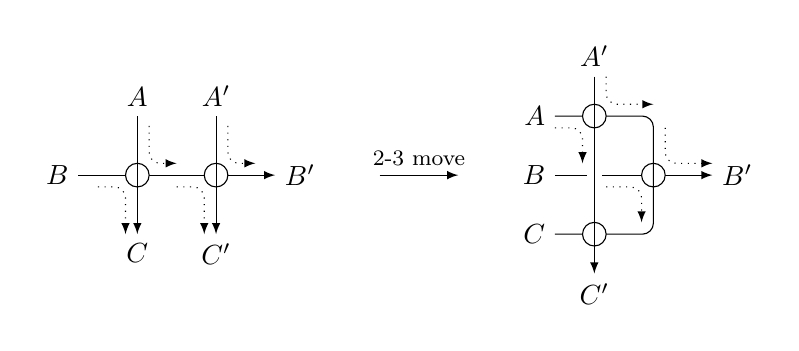
\begin{tikzpicture}[> = latex]
\matrix[column sep = 0.5 cm, row sep = 0.5 cm]{

	% 2-vertex subgraph with Eulerian circuit

	\draw [->] (-1.25, 0) node [left] {$B$} -- (1.25, 0) node [right] {$B'$};

	\draw [fill = white] (-0.5, 0) circle (0.15);
	\draw [fill = white] (0.5, 0) circle (0.15);

	\draw [->] (-0.5, 0.75) node [above] {$A$} -- (-0.5, -0.75) node [below] {$C$};
	\draw [->] (0.5, 0.75) node [above] {$A'$} -- (0.5, -0.75) node [below] {$C'$};

	% Internal connections
	
	\begin{scope}[->, dotted, rounded corners]
	
		\draw (-0.35, 0.625) -- (-0.35, 0.15) -- (0, 0.15);
		\draw (-1, -0.15) -- (-0.65, -0.15) -- (-0.65, -0.75);
		
		\draw (0, -0.15) -- (0.35, -0.15) -- (0.35, -0.75);
		\draw (0.65, 0.625) -- (0.65, 0.15) -- (1, 0.15);
	
	\end{scope}

&

	\draw [->, font = \footnotesize] (0, 0) -- node [above] {2-3 move} (1, 0);

&

	% 3-vertex subgraph

	\draw [->] (-0.5, 0) node [left] {$B$} -- (1.5, 0) node [right] {$B'$};
	\draw [fill = white] (0.75, 0) circle (0.15);

	\draw [rounded corners] (-0.5, 0.75) node [left] {$A$} -- (0.75, 0.75) -- (0.75, -0.75) -- (-0.5, -0.75) node [left] {$C$};

	\draw [fill = white] (0, 0.75) circle (0.15);
	\draw [fill = white] (0, -0.75) circle (0.15);

	\draw (0, 1.25) node [above] {$A'$} -- (0, 0.35);
	\draw [draw = white, double = black, double distance between line centers = 3 pt, line width = 2.6 pt] (0, 0.35)  -- (0, -0.35);
	\draw [<-] (0, -1.25) node [below] {$C'$} -- (0, -0.35);

	% Internal connections
	
	\begin{scope}[->, dotted, rounded corners]
	
		\draw (0.15, 1.25) -- (0.15, 0.9) -- (0.75, 0.9);
		\draw (-0.5, 0.6) -- (-0.15, 0.6) -- (-0.15, 0.15);
		
		\draw (0.15, -0.15) -- (0.6, -0.15) -- (0.6, -0.6);
		\draw (0.9, 0.6) -- (0.9, 0.15) -- (1.5, 0.15);
	
	\end{scope}

\\
};
\end{tikzpicture}

\end{document}